\newcommand{\lsthaskell}[1]{\lstinline[language=haskell]{#1}}
\newcommand{\Q}{{\color{red}Q:}\hspace{2mm}}
\newcommand{\A}{{\color{blue}A:}\hspace{2mm}}

\begin{frame}{A parser in 22 questions}
  Define a parser for arithmetic expressions in a series of questions.

\[
  t ::= \langle number \rangle ~|~ ( t ) ~|~ t + t ~|~ t - t ~|~ t * t ~|~ t / t
\]

  \begin{itemize}
  \item{{\bf Goal:} avoid the usual problems with parsing:\\
      associativity, precedence, left-recursion, detecting and
      resolving ambiguity, etc}
  \item{{\bf Idea:} use input/output examples as specification}

  \item{{\bf Idea:} system detects what it needs to know how to parse,
      and asks for examples}
\end{itemize}
\end{frame}

\begin{frame}[fragile]
\frametitle{First Steps}

  Start by defining the Abstract Syntax Tree (mirrors the BNF):

\begin{center}
\begin{minipage}{.7\textwidth}
$t ::= \langle number \rangle ~|~ ( t ) ~|~ t + t ~|~ t - t ~|~ t * t ~|~ t / t$

\begin{lstlisting}[mathescape,language=haskell]
data T = Num Int | Paren T
       | Add T T | Sub T T
       | Mul T T | Div T T

parseT :: String $\to$ T
parseT = ???
\end{lstlisting}
\end{minipage}
\end{center}

\begin{itemize}
\item{The type T defines the possible syntactic cases in our language,
    used to determine whether a specification is complete.}
\item{$parse$ is the parser we want to synthesize.}
\end{itemize}
\end{frame}

\begin{frame}[fragile]
\frametitle{Bootstrapping Examples}
  Interactive Q/A session (22 questions in this case):

\begin{itemize}
  \item A ``bootstrapping'' example for each case (6 examples)
  \item {Detect and resolve ambiguities:
    \begin{itemize}
      \item Associativity of each operator (4 examples)
      \item Precedence rules (12 examples)
    \end{itemize}
  }
\end{itemize}

\end{frame}

\begin{frame}[fragile]
\frametitle{Bootstrapping Examples}

\begin{itemize}
\item Collect small examples of each case
\item Generalize to produce an initial specification
\end{itemize}

\vspace{5mm}

\Q Does ``123'' parse as \lsthaskell{Num 123}? (Y/N)\\
\A Y
\vspace{2mm}

\Q Which input parses as \lsthaskell{Paren (Num 0)}?\\
\A ``(0)''\\
\vspace{2mm}

\Q Which input parses as \lsthaskell{Add (Num 1) (Num 2)}?\\
\A ``1+2''\\
\vspace{2mm}

\Q Which input parses as \lsthaskell{Sub (Num 1) (Num 2)}?\\
\A ``1-2''\\

$\dots$

\end{frame}

\begin{frame}[fragile]
\frametitle{Detecting Ambiguity}

The specification can be used to synthesize a {\em pretty-printer},
which {\em must be} the right inverse of a parser:

\begin{lstlisting}[mathescape, language=haskell]
print :: T -> String
$\forall$t:T. parse (print t) == t
\end{lstlisting}

\begin{itemize}
\item{\lsthaskell{print} must be one-to-one}
\item{If \lsthaskell{print} maps two distinct ASTs to the same
    string, our specification is ambiguous}
\item{Automatically detect ambiguities (e.g. systematic search)}
\item{Ask questions to resolve them}
\end{itemize}
\end{frame}

\begin{frame}[fragile]
\frametitle{Resolving Ambiguities}

\begin{itemize}
\item Ask user to choose between possible parses of a string
\end{itemize}

\vspace{5mm}

\Q What is the parse of ``1+2*3''? \hspace{2mm} (A/B)

\hspace{6mm}\begin{minipage}{.4\textwidth}
{\bf Choice A:}\\
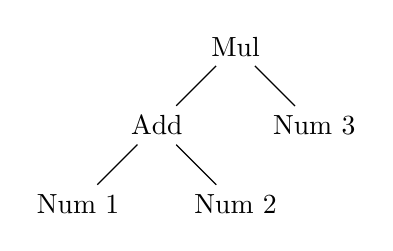
\begin{tikzpicture}
  \node(root) at (3,3){Mul};
  \node(l) at (2,2){Add};
  \node(ll) at (1,1){Num 1};
  \node(lr) at (3,1){Num 2};
  \node(r) at (4,2){Num 3};

  \draw (root) -- (l);
  \draw (root) -- (r);
  \draw (l) -- (ll);
  \draw (l) -- (lr);
\end{tikzpicture}
\end{minipage}
\hspace{5mm}
\begin{minipage}{.4\textwidth}
{\bf Choice B:}\\
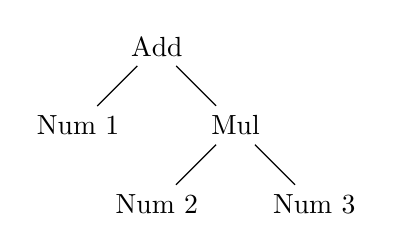
\begin{tikzpicture}
  \node(root) at (3,3){Add};
  \node(l) at (2,2){Num 1};
  \node(r) at (4,2){Mul};
  \node(rl) at (3,1){Num 2};
  \node(rr) at (5,1){Num 3};

  \draw (root) -- (l);
  \draw (root) -- (r);
  \draw (r) -- (rl);
  \draw (r) -- (rr);
\end{tikzpicture}
\end{minipage}
\\
\A B
\vspace{2mm}

\begin{itemize}
\item{Choice A flagged as an invalid AST (can't be printed)}
\item{Similar questions resolve all associativity and precedence
    ambiguities}
\end{itemize}
\end{frame}

\begin{frame}[fragile]
\frametitle{The complete {\small(abridged)} specification}

\begin{itemize}
\item{In 22 examples}
\end{itemize}

\begin{lstlisting}[mathescape,language=haskell]
-- bootstrapping
parse "123" == Num 123
parse "(0)" == Paren (Num 0)
parse "1+2" == Add (Num 1) (Num 2)   (x4)

-- associativity
parse "1+2+3" == 
  Add (Add (Num 1) (Num 2)) (Num 3)  (x4)

-- precedence
parse "1+2*3" == 
  Add (Num 1) (Mul (Num 2) (Num 3))  (x12)
\end{lstlisting}

\end{frame}